\documentclass{article}
\usepackage{graphicx}
\usepackage{xcolor}
\usepackage{amsmath}
\usepackage{amssymb}
\usepackage{authblk}
\usepackage{subcaption}
\usepackage{float}
\usepackage{placeins}
\usepackage{booktabs}
\usepackage{pdflscape}
\usepackage[numbers]{natbib}
\usepackage{setspace}
\usepackage{parskip}
\usepackage{microtype}
\usepackage[margin=2.5cm]{geometry}

\setlength{\parindent}{0pt}
\setlength{\parskip}{7pt}
\linespread{1.15}

\newcommand{\PCAVarI}{46.8\%}
\newcommand{\PCAVarII}{28.0\%}
\newcommand{\PCAVarTotal}{74.8\%}

\title{\textbf{Neural Population Dynamics Reveal Internal Representations
Underlying Adaptive Obstacle Avoidance in Reinforcement Learning}}

\author[1]{Peter Ohue}
\author[1]{Emily Oby}
\author[1,2]{Gunnar Blohm}

\affil[1]{Centre for Neuroscience Studies, Queen's University, ON, Canada}
\affil[2]{Department of Biomedical and Molecular Sciences,
          Queen's University, ON, Canada}

\date{}

\begin{document}

\maketitle

%--------------------------------------------------------------
\begin{abstract}
%--------------------------------------------------------------

Adaptive motor control under unexpected mechanical perturbation requires the
rapid generation of corrective responses that maintain goal-directed movement
without disrupting kinematic efficiency.
Understanding what internal computational signals drive these corrections, and
what determines whether a controller recovers or fails, remains a fundamental
challenge in both systems neuroscience and autonomous motor control, in part
because the relevant signals are not directly accessible from behavioural
measurements alone.
We developed a computational framework that places a reinforcement learning
controller, trained through the same trial-and-error refinement that shapes
biological motor learning, in a reaching-inspired obstacle-avoidance task and
challenges it with graded lateral force impulses, mirroring protocols used to
study feedback correction in human arm movements.
Rather than reporting only task success, we record the controller's
hidden-layer activity during evaluation and treat it as a neural population
signal, applying dimensionality reduction, state-space trajectory analysis,
and linear decoding to ask what internal representations track behaviour
and distinguish recovery from failure.

We find that the controller adapts successfully to moderate perturbations
across all directions but fails progressively under strong rightward
disturbances, revealing a direction-dependent asymmetry in robustness that
traces back to the geometry of the learned corridor trajectory.
The hidden-layer activity organises into a compact low-dimensional manifold,
with the large majority of population variance captured in just two principal
components, and subdivides into four discrete clusters that correspond to
phases of the movement rather than to specific perturbation conditions.
Lateral velocity is clearly and systematically encoded across the
population, and the most extreme perturbation conditions produce latent
states that a simple linear classifier can separate from one another,
while mild conditions remain geometrically indistinct because they generate
similar corrective responses.
These properties closely parallel those documented in motor cortex during
biological reaching: compact manifold geometry, phase-structured clustering,
and distributed, linearly readable encoding of kinematic variables.
Our results suggest that reward-driven optimisation spontaneously generates
representational organisation that is functionally similar to what has
been found in biological motor populations, and that population-style
analyses of artificial controllers can reveal not just whether adaptive
behaviour succeeds but, mechanistically, why it sometimes does not.

\end{abstract}

%==============================================================
\section{Introduction}
%==============================================================

The ability to reach toward a target while correcting for unexpected
mechanical disturbances is one of the defining capacities of the biological
motor system \citep{Pruszynski2012,Nashed2014,Dimitriou2013,Scott2004}.
When the moving limb is deflected by an external force, the nervous system
does not pause for deliberate decision-making; rapid feedback corrections
emerge within tens of milliseconds, coordinated by the
continuous interplay between sensory inflow and internal predictions about
the limb's future state
\citep{Todorov2002,Todorov2009,Codol2023,FlashHogan1985}.
Critically, this flexibility does not reside in individual neurons.
It emerges from coordinated activity across distributed populations in
motor cortex and cerebellum, populations whose collective dynamics
constitute a low-dimensional trajectory through a high-dimensional
activity space
\citep{Churchland2012,Shenoy2013,Gallego2017,Crevecoeur2019,Blohm2009,Georgopoulos1986,Kalaska1989}.
Understanding how this population-level organisation gives rise to robust,
adaptive behaviour is a central goal of systems motor neuroscience.

Reinforcement learning (RL) offers a complementary computational
perspective on the same problem.
In RL, a controller is not given explicit movement rules; instead, it
discovers a control policy through repeated interaction with an environment,
receiving a scalar reward whenever it performs well and adjusting its
internal parameters accordingly
\citep{Kaelbling1996RLSurvey,SuttonBarto2018,Schulman2017}.
This reward-driven learning is, in spirit, analogous to biological motor
skill acquisition: practice generates sensory and outcome feedback, and the
nervous system gradually refines its internal representation to maximise
successful performance \citep{Oby2019,Mathis2024,Shadmehr1994,WolpertGhahramani2000,Krakauer2019}.
The comparison is not merely metaphorical; both processes involve an agent
updating a policy based on signals about the quality of recent actions,
without being told what the correct movement should have been.

Proximal Policy Optimization (PPO) \citep{Schulman2017}, the algorithm
used here, is a widely adopted policy-gradient method whose update rule is
designed to prevent destabilising changes to the learned policy.
At each training iteration, PPO estimates the relative performance of a
proposed policy update against the current policy and restricts the update
to a bounded neighbourhood around the existing solution, clipping the
probability ratio to the interval $[1-\epsilon, 1+\epsilon]$.
This constraint formalises a principle well-established in motor learning
research: incremental, bounded refinement of the control policy is more
stable than wholesale revision, because large parameter changes risk
degrading performance that has already been acquired \citep{Oby2019,SuttonBarto2018,Heald2021,Krakauer2019}.
The term ``proximal'' refers precisely to this neighbourhood constraint:
updates stay close to the current policy, producing steady improvement
without the catastrophic performance swings that unconstrained gradient
ascent can generate.

Despite strong task performance, most RL studies evaluate controllers
solely on behavioural outcomes such as success rate, cumulative reward,
and mean path length, treating the policy network as a black box
\citep{Rudin2019,Molnar2022}.
This characterisation is informative but mechanistically incomplete: it
cannot explain which internal signals distinguish a trial in which the
agent successfully corrects from one that ends in collision.
Identifying such signals is precisely the kind of question that
population-level analyses have addressed in biological motor cortex
\citep{Churchland2012,Cunningham2014,Gallego2017,Blohm2009}.

Population activity in motor cortex during reaching evolves along smooth,
low-dimensional neural manifolds, defined as compact subspaces within the
high-dimensional activity space that capture the essential structure of
movement generation
\citep{Churchland2012,Shenoy2013,Cunningham2014,Gallego2017,Sadtler2014,Elsayed2016,Kaufman2014}.
Individual neurons within these populations exhibit heterogeneous tuning
to kinematic variables, but the population as a whole encodes these
variables in a structured, often linearly readable form
\citep{Oby2019,Blohm2009,Georgopoulos1986,Perich2018}.
These observations motivate the central question of this study: does an
artificially trained controller that was never designed to resemble a
biological motor system develop similar representational organisation as a
natural consequence of reward-driven learning?

We train a PPO controller on a two-dimensional obstacle-avoidance reaching
task and evaluate it under seven graded perturbation conditions spanning
both directions of lateral displacement, mirroring designs used in human
perturbation studies.
During evaluation, we extract the hidden-layer activations of the policy
network at every timestep and treat the resulting collection as a
population recording.
We then apply principal component analysis (PCA) to reveal the geometry
of the latent state space, examine the relationship between individual
unit activity and instantaneous lateral velocity, and train linear
classifiers to test whether perturbation context can be read directly
from single-timestep population activity.

Our contributions are four-fold.
First, we demonstrate a population-analysis workflow for trained RL
controllers that enables direct comparison with biological motor data.
Second, we show that the controller's hidden-layer activity exhibits
compact low-dimensional manifold structure consistent with neural manifold
dynamics in motor cortex.
Third, we identify a direction-dependent asymmetry in robustness, whereby
rightward perturbations prove more disruptive than leftward ones of equal
magnitude, visible in both behaviour and latent geometry.
Fourth, we show that extreme perturbation conditions produce linearly
separable latent representations while mild ones do not, mirroring the
difficulty-dependent separability observed in biological neural population
studies.


%==============================================================
\section{Methodology}
%==============================================================

\subsection{Task Environment}

We implemented the obstacle-avoidance environment using the Gymnasium
interface \citep{Towers2024Gymnasium}, a standard open-source framework
for defining physics-based reinforcement learning environments.
The agent is a two-dimensional point mass that receives continuous force
commands at each timestep and evolves under Newtonian dynamics within a
bounded rectangular workspace.
We deliberately kept the dynamics minimal (a single point mass with no
rotational degrees of freedom and no joint limits) so that any
representational structure found in the trained network is attributable
to learning rather than to the complexity of the physical system.
This minimalism also makes the setup directly comparable to the planar
arm-perturbation paradigms used in human motor neuroscience, where the
task geometry rather than the limb dynamics is the primary independent
variable \citep{Nashed2014,Pruszynski2012,Shadmehr1994,Franklin2011}.

Figure~\ref{fig:schematic} illustrates the task and analysis pipeline.
Panel~A uses a planar arm and brain schematic to connect the setup to the
biological literature; all experiments use the point-mass dynamics
summarized in Panel~C.
Panel~B shows the PPO actor--critic loop that governs learning.

\begin{figure}[H]
  \centering
  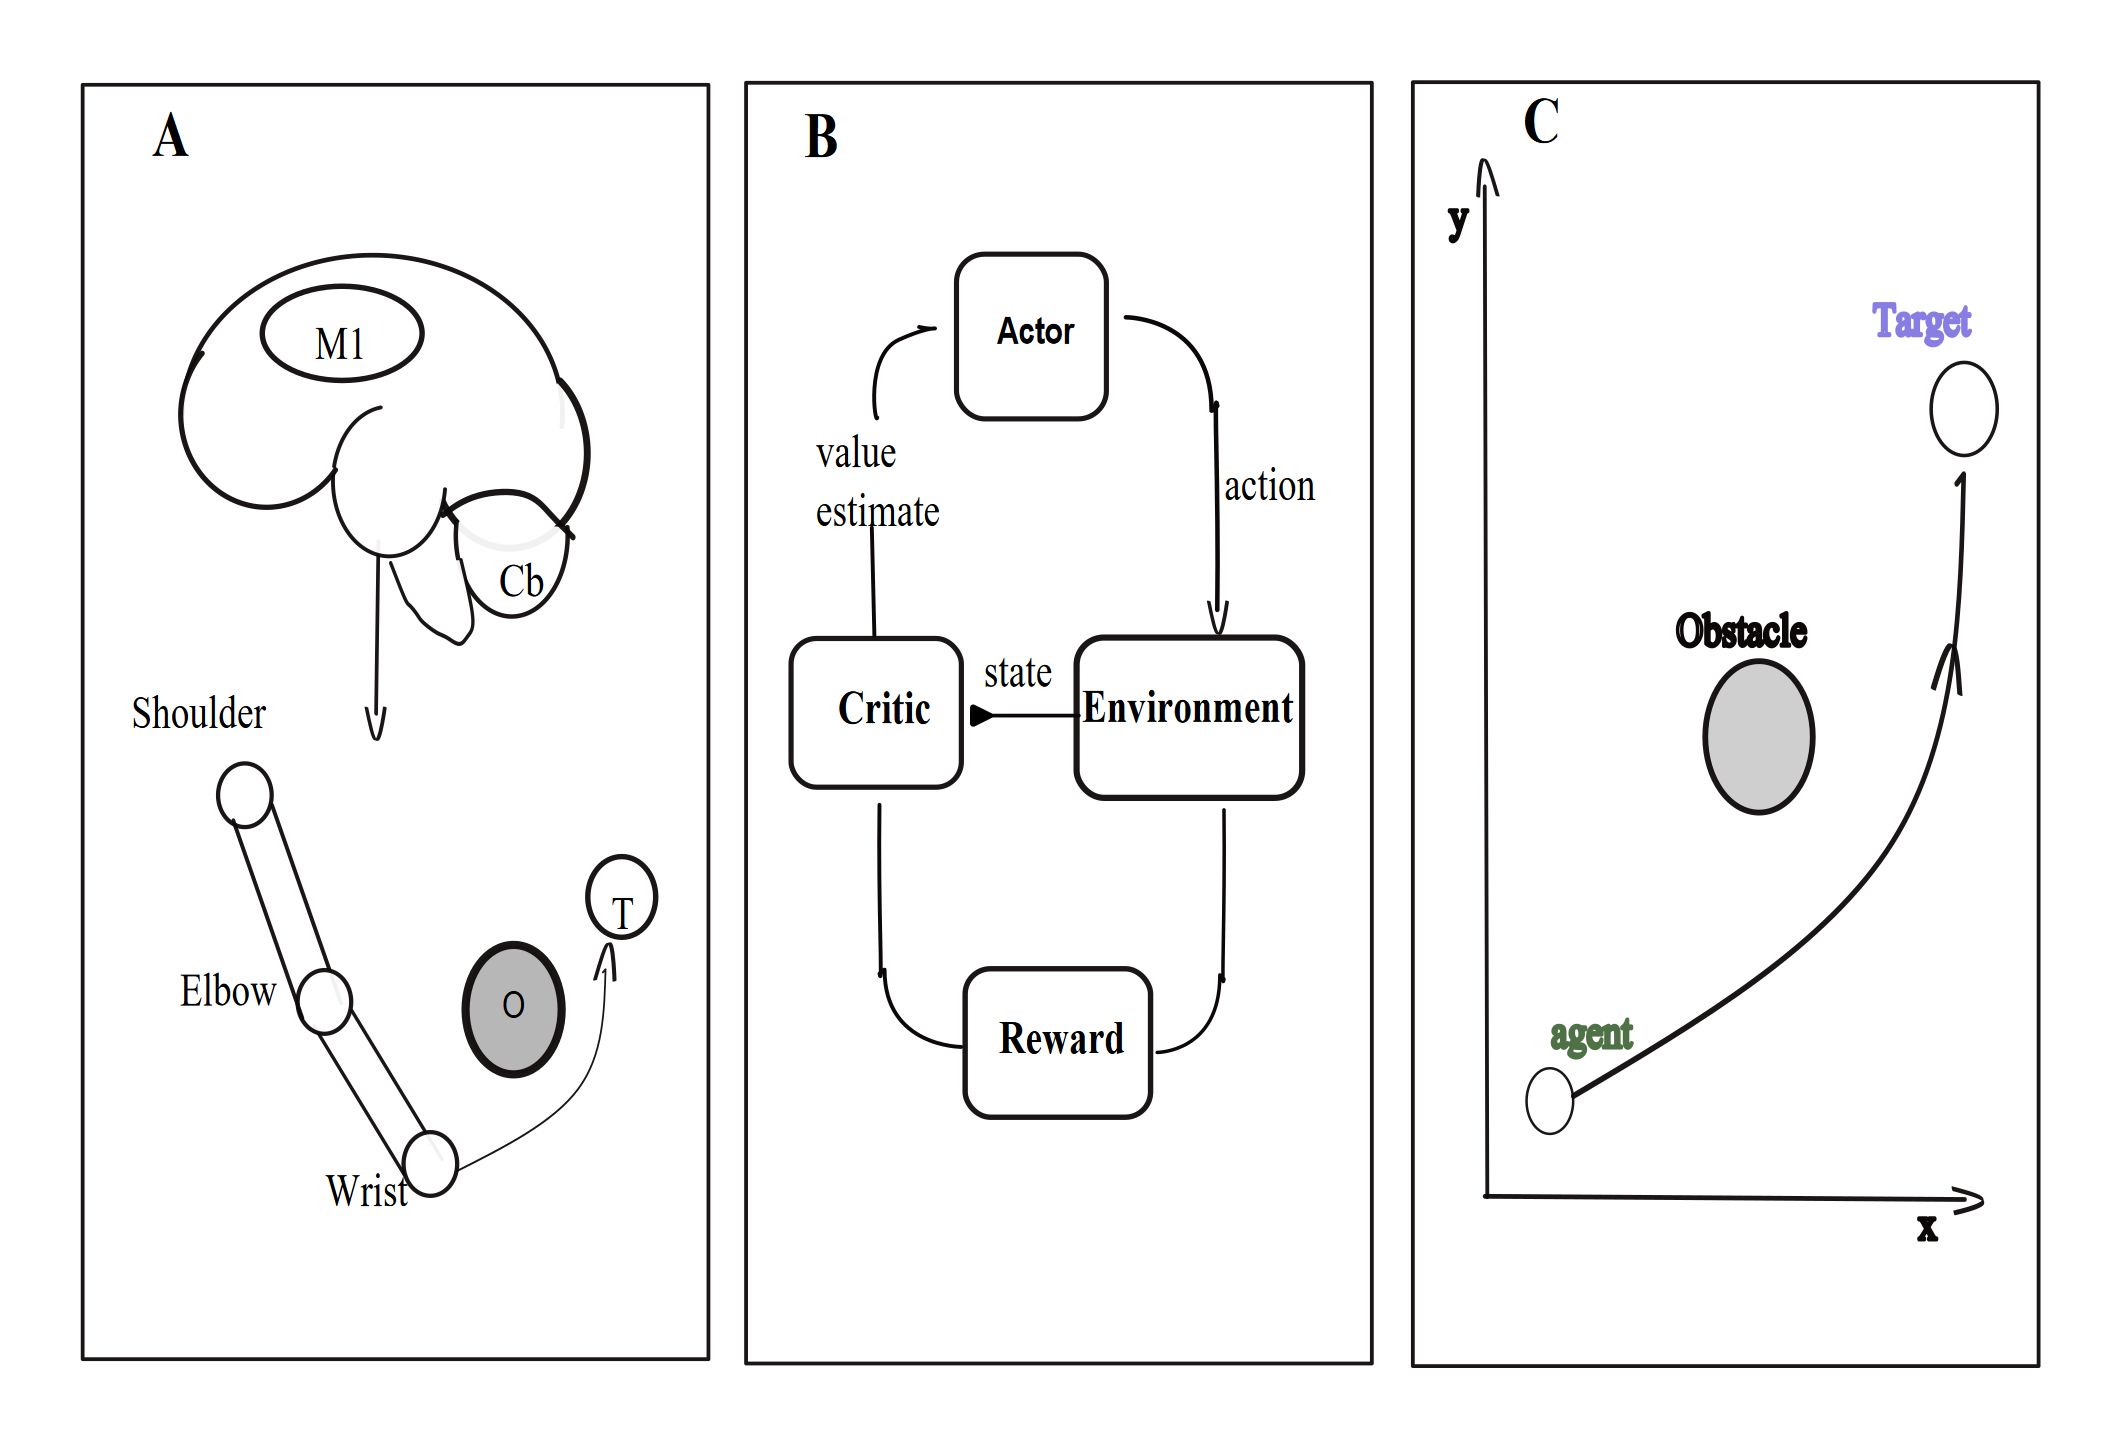
\includegraphics[width=0.88\linewidth]{fig1_schematic.png}
  \caption{\textbf{Task design, control architecture, and population
    analysis pipeline.}
    \textbf{(A)}~Biological analogy illustrating the conceptual parallel
    between the artificial controller and biological motor control.
    Primary motor cortex (M1) provides descending drive to the shoulder,
    elbow, and wrist, guided by cerebellar (Cb) predictions and sensory
    feedback, to move a multi-joint arm toward a target~(T) while avoiding
    an obstacle~(O). This panel situates the computational setup in the
    language of systems motor neuroscience; the actual experiments use a
    point-mass agent.
    \textbf{(B)}~The PPO actor--critic control loop. At each timestep,
    the \emph{actor} network receives the current state observation and
    outputs a continuous force command (the action). The
    \emph{environment} applies that command, advances the agent one
    timestep, and returns the new state. The \emph{critic} network
    receives the state and estimates its long-term value; together with the
    observed reward, this estimate is used to compute the advantage that
    guides the actor's update. A scalar reward signal is produced
    by the environment at every timestep to drive both networks.
    \textbf{(C)}~Task geometry. The agent (green dot) starts at a fixed
    position at the bottom of the workspace and must navigate to a fixed
    goal (top) on a two-dimensional Cartesian plane, while avoiding
    the obstacle(s) in the corridor between start and goal.}
  \label{fig:schematic}
\end{figure}

The main perturbation experiment used a corridor formed by two static
circular obstacles positioned symmetrically about the midline of the
workspace.
The corridor is narrow enough that trajectories deflected by strong lateral
perturbations risk collision with one of the obstacle boundaries, making
it a sensitive test of online correction ability.
A preliminary single-obstacle experiment was run first to establish the
basic obstacle-avoidance skill; the two-obstacle configuration was then
introduced and training continued until performance plateaued.

\subsection{State Representation}

The agent's observation at each timestep provides a complete description
of the task-relevant geometry in agent-centred coordinates:
\begin{equation}
  s_t = \bigl[
    g_x - x_t,\;g_y - y_t,\;
    o_{Lx} - x_t,\;o_{Ly} - y_t,\;
    o_{Rx} - x_t,\;o_{Ry} - y_t,\;
    v_{x,t},\;v_{y,t}
  \bigr]
  \label{eq:state}
\end{equation}
where $(x_t,y_t)$ is the agent's current position, $(v_{x,t},v_{y,t})$
its current velocity, $(g_x,g_y)$ the goal location, and $(o_L,o_R)$ the
centres of the left and right obstacles.
Expressing all spatial quantities relative to the agent rather than in
absolute workspace coordinates renders the representation invariant to the
agent's absolute position, which reduces the effective dimensionality of
the learning problem and encourages the development of generalizable
movement policies.

\subsection{Reward Function}

The agent receives a scalar reward at each timestep that encodes four
distinct objectives:
\begin{equation}
  R_t = w_p\,\Delta d_{\mathrm{goal}}
        - w_v\,\|v_t\|
        - w_c\,C_t
        + w_s\,S_t
  \label{eq:reward}
\end{equation}
The first term rewards reduction in the Euclidean distance to the goal
($\Delta d_{\mathrm{goal}} > 0$ when the agent moves closer);
the second penalises excessive instantaneous speed to encourage smooth
movements;
the third imposes a large negative penalty upon collision with an obstacle
($C_t = 1$ at collision, $0$ otherwise);
and the fourth provides a terminal bonus upon successful goal attainment
($S_t = 1$ at success, $0$ otherwise).
The weights $w_p, w_v, w_c, w_s$ were tuned so that efficient goal-seeking
was the dominant objective while collision avoidance remained a hard
constraint in practice.

\subsection{Perturbation Protocol}

To probe the controller's capacity for online correction, we applied
transient lateral force impulses mid-movement during evaluation.
The impulse magnitude was held constant for six consecutive timesteps
beginning at timestep 50:
\begin{equation}
  f_x(t) = p_i, \quad t \in [50,\,55], \quad
  p_i \in \{\pm0.15,\;\pm0.30,\;\pm0.45\}
  \label{eq:perturbation}
\end{equation}
A positive value of $p_i$ corresponds to a rightward impulse; a negative
value to a leftward impulse.
This yields seven evaluation conditions: an unperturbed control (P0) and
three increasing leftward perturbations (L1: $-0.15$, L2: $-0.30$, L3:
$-0.45$) and three increasing rightward perturbations (R1: $+0.15$, R2:
$+0.30$, R3: $+0.45$).
The six-timestep impulse window is brief relative to the typical episode
duration (approximately 100--120 timesteps), mimicking the short-duration
mechanical perturbations applied in biological reaching paradigms to
isolate online feedback responses from anticipatory motor planning
\citep{Pruszynski2012,Nashed2014,Dimitriou2013,Todorov2002,Shadmehr1994}.

\subsection{Reinforcement Learning Controller and Training}

All training and evaluation used Stable-Baselines3
\citep{Raffin2021StableBaselines3}, an open-source Python library built
on PyTorch that provides rigorously tested implementations of standard
deep RL algorithms.
We used Proximal Policy Optimization (PPO) \citep{Schulman2017}, which
maximises the following clipped surrogate objective:
\begin{equation}
  L^{\mathrm{CLIP}}(\theta) = \mathbb{E}_t\!\Bigl[
    \min\!\bigl(r_t(\theta)\hat{A}_t,\;
    \mathrm{clip}(r_t(\theta),1-\epsilon,1+\epsilon)\hat{A}_t\bigr)
  \Bigr]
  \label{eq:ppo}
\end{equation}
Here $r_t(\theta) = \pi_\theta(a_t|s_t) / \pi_{\theta_{\mathrm{old}}}(a_t|s_t)$
is the probability ratio of the new policy to the old policy,
$\hat{A}_t$ is the generalized advantage estimate (a measure of how much
better the selected action was relative to the expected value of that
state), and $\epsilon = 0.2$ is the clipping parameter that restricts
the policy ratio to the interval $[1-\epsilon, 1+\epsilon]$, bounding
the size of any single update step.

The policy and value networks are separate feedforward multilayer
perceptrons (MLPs), each with two hidden layers of 256 units and
rectified linear (ReLU) activations.
A feedforward MLP processes each timestep independently, without recurrence
or explicit memory of previous states.
Continuous actions are drawn from a diagonal Gaussian distribution whose
mean is output by the actor network; the standard deviation is a learned
parameter.
Observations were standardised online using a running mean and variance
(VecNormalize), which substantially improves training stability in
continuous-control settings.
Training ran for $3\times10^6$ environment timesteps with the following
hyperparameters: learning rate $\alpha = 3\times10^{-4}$, discount factor
$\gamma = 0.99$, generalised advantage estimation parameter
$\lambda_{\mathrm{GAE}} = 0.95$, entropy regularisation coefficient
$c_{\mathrm{ent}} = 0.005$, value-function loss coefficient $c_v = 0.5$,
and maximum gradient norm $0.5$.
All experiments were run with Stable-Baselines3 v2.8.0, Gymnasium,
and PyTorch on an Intel\textregistered\ Core\textsuperscript{TM} Ultra~7~255H
processor.

\subsection{Neural Population Analysis Pipeline}

Following training convergence, we extracted the activation vector
$h_t \in \mathbb{R}^{256}$ from the first hidden layer of the policy
network at every timestep $t$ of every evaluation episode.
Let $T$ denote the length of an episode; the full population record for
that episode is:
\begin{equation}
  H = \{h_1, h_2, \ldots, h_T\}
  \label{eq:latent}
\end{equation}
Concatenating $H$ across all evaluation episodes gives a matrix of
shape $N_{\mathrm{total}} \times 256$, where $N_{\mathrm{total}}$ is the
total number of timesteps across all episodes and conditions.

Three population-level analyses were then applied to this matrix.

\textbf{Principal Component Analysis (PCA).}
PCA finds a set of orthogonal directions, called principal components, that
account for successively decreasing fractions of the total variance in
the population data.
Projecting the 256-dimensional activity onto the first two principal
components provides a two-dimensional visualisation of the population
state space and allows us to quantify how compactly the activity is
organised.
We report the fraction of total variance explained by each principal
component as a direct measure of dimensionality compression.

\textbf{Kinematic tuning analysis.}
For each of the 256 hidden units, we computed the Pearson correlation
between its activation and instantaneous lateral velocity across all
evaluation timesteps.
This identifies units that are systematically modulated by the direction
or magnitude of lateral movement, analogous to single-unit tuning analyses
in biological motor electrophysiology.

\textbf{Linear decoding.}
We trained a multinomial logistic regression classifier (regularisation
$C = 1.0$) on single-timestep hidden-layer activity to predict which of
the seven perturbation conditions was active.
A linear classifier was used deliberately: if strong decoding performance
can be achieved with a linear readout, it implies that the relevant
information is encoded in the geometry of the population activity in a
relatively direct, structured way rather than requiring nonlinear
transformations to extract.
Classifier performance is summarised as a confusion matrix across
conditions.
All analyses were implemented in Python using NumPy, SciPy, and
scikit-learn.

%==============================================================
\section{Results}
%==============================================================

We evaluated the trained PPO controller across all seven perturbation
conditions (P0, L1--L3, R1--R3) and report findings in four parts,
proceeding from observable behaviour to the internal representations that
underlie it.

Figure~\ref{fig:trajectories} shows cumulative reach trajectories
overlaid across all seven perturbation conditions.
In the unperturbed control (P0) and all mild conditions (L1, L2, R1),
the controller reached the goal on every evaluation trial, generating
smooth, roughly symmetric paths that arced around both obstacles.
As perturbation magnitude increased, trajectories deflected progressively
in the direction of the applied force: leftward conditions (L1--L3) bowed
the path toward the left obstacle; rightward conditions (R1--R3) bowed it
toward the right.

\begin{figure}[H]
  \centering
  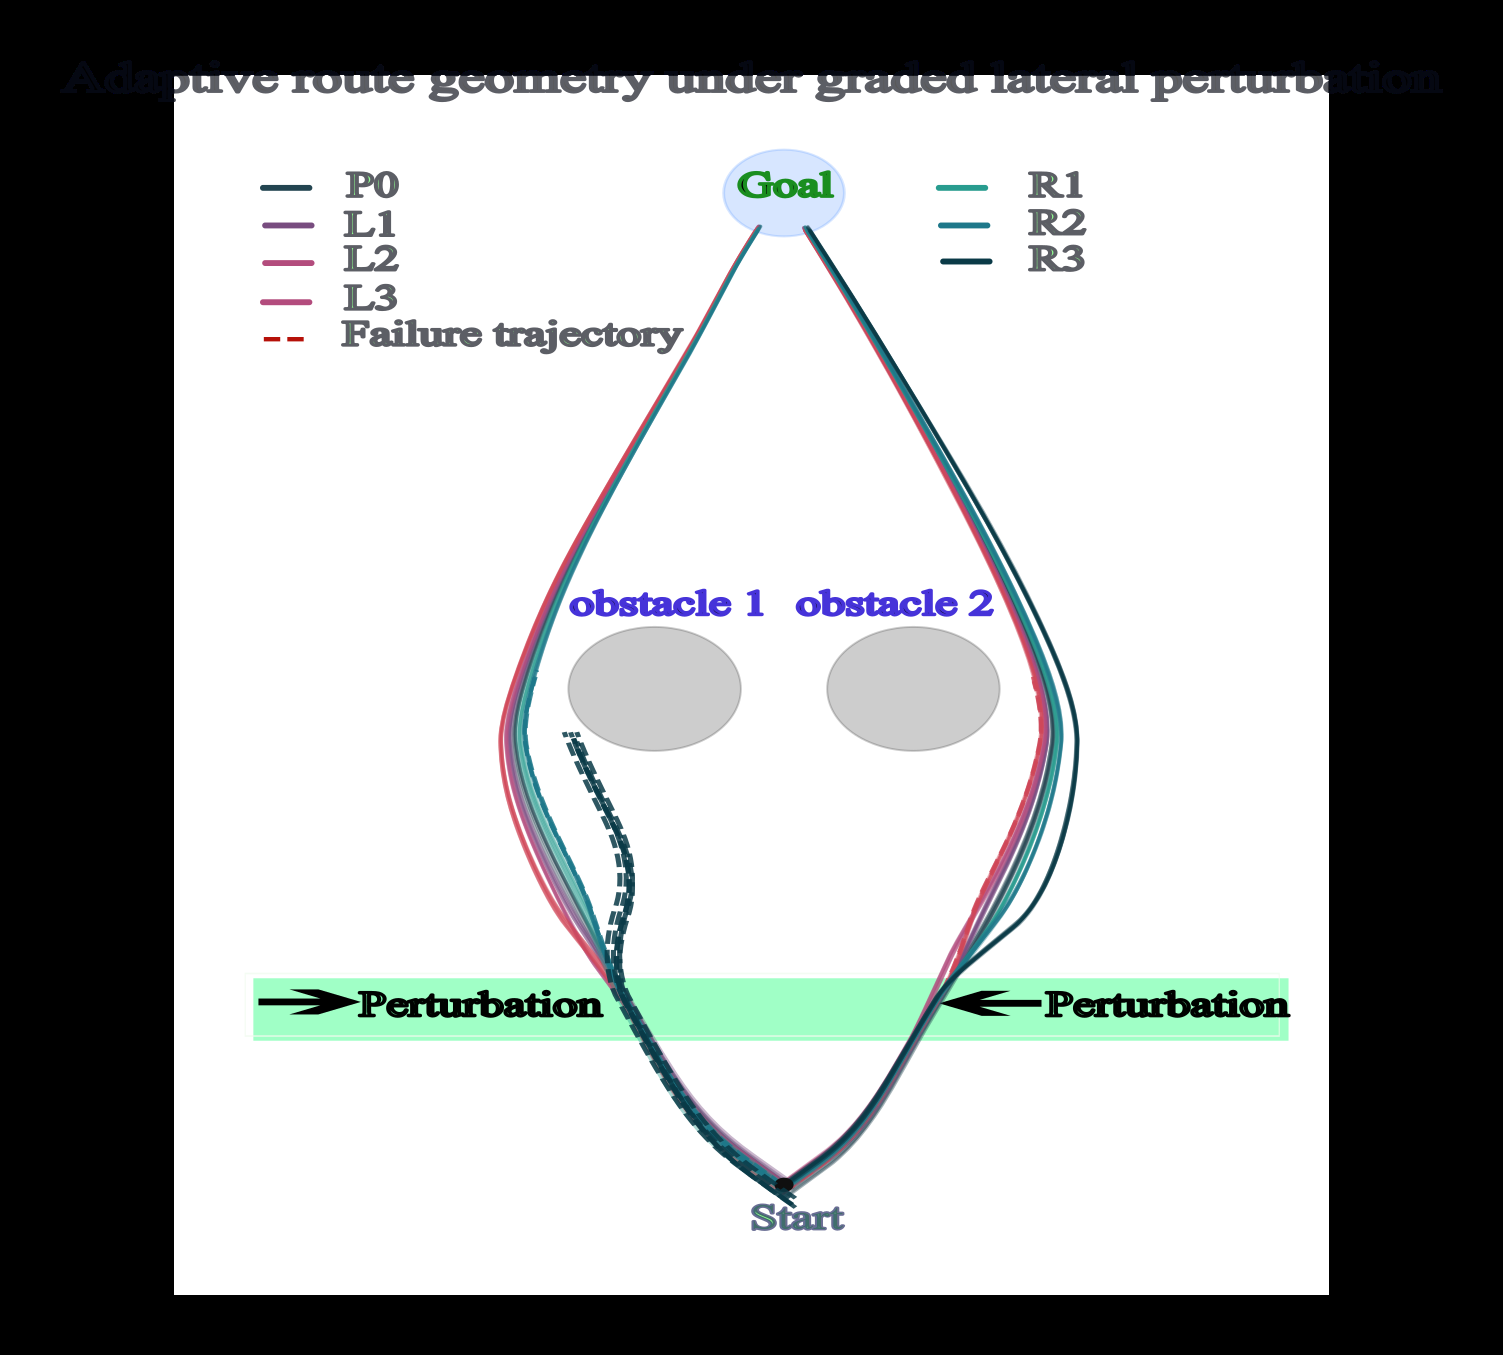
\includegraphics[width=0.58\linewidth]{fig2_trajectories.png}
  \caption{\textbf{Cumulative reach trajectories across all seven
    perturbation conditions illustrating the limits of adaptive correction.}
    Each evaluation episode is overlaid separately for each condition.
    Solid lines are successful trials that reached the goal; the dashed
    red lines are failure trajectories that ended in obstacle collision.
    Leftward perturbation conditions (L1--L3, mauve/pink tones) progressively
    deflect the path toward the left obstacle, while rightward conditions
    (R1--R3, teal/dark green) deflect it toward the right.
    The shaded green horizontal band marks the region of the workspace in
    which the lateral force impulse is active (timesteps 50--55), providing
    a reference for when in the movement the perturbation is applied.
    Grey ellipses represent the two static obstacles forming the corridor.
    The controller maintained complete goal success under control and all
    mild conditions; success declined only under the two strongest rightward
    disturbances and under the largest leftward impulse, with rightward
    perturbations proving disproportionately disruptive, a geometric
    consequence of the controller having learned a trajectory that runs
    slightly to the left of corridor centre.}
  \label{fig:trajectories}
\end{figure}

Goal success declined only at the two strongest rightward magnitudes
(R2 and R3) and at the largest leftward magnitude (L3).
Notably, rightward perturbations were more disruptive than leftward ones
of the same nominal force.
This directional asymmetry is a geometric consequence of the learned
trajectory: the controller settles on a path that runs slightly to the
left of the corridor midline, giving it more clearance from the left
obstacle and less from the right.
An equivalent rightward push therefore risks collision with the right
obstacle before a sufficient correction can be generated, while an
equivalent leftward push carries the agent away from the right obstacle
into a region with more room to correct.
Across all successful trials, peak speed was effectively constant across
conditions; adaptation was expressed entirely through lateral path geometry,
not through modulation of movement tempo.

Figure~\ref{fig:velocity} characterises the temporal evolution of
lateral velocity and total speed across all seven conditions.

\begin{figure}[H]
  \centering
  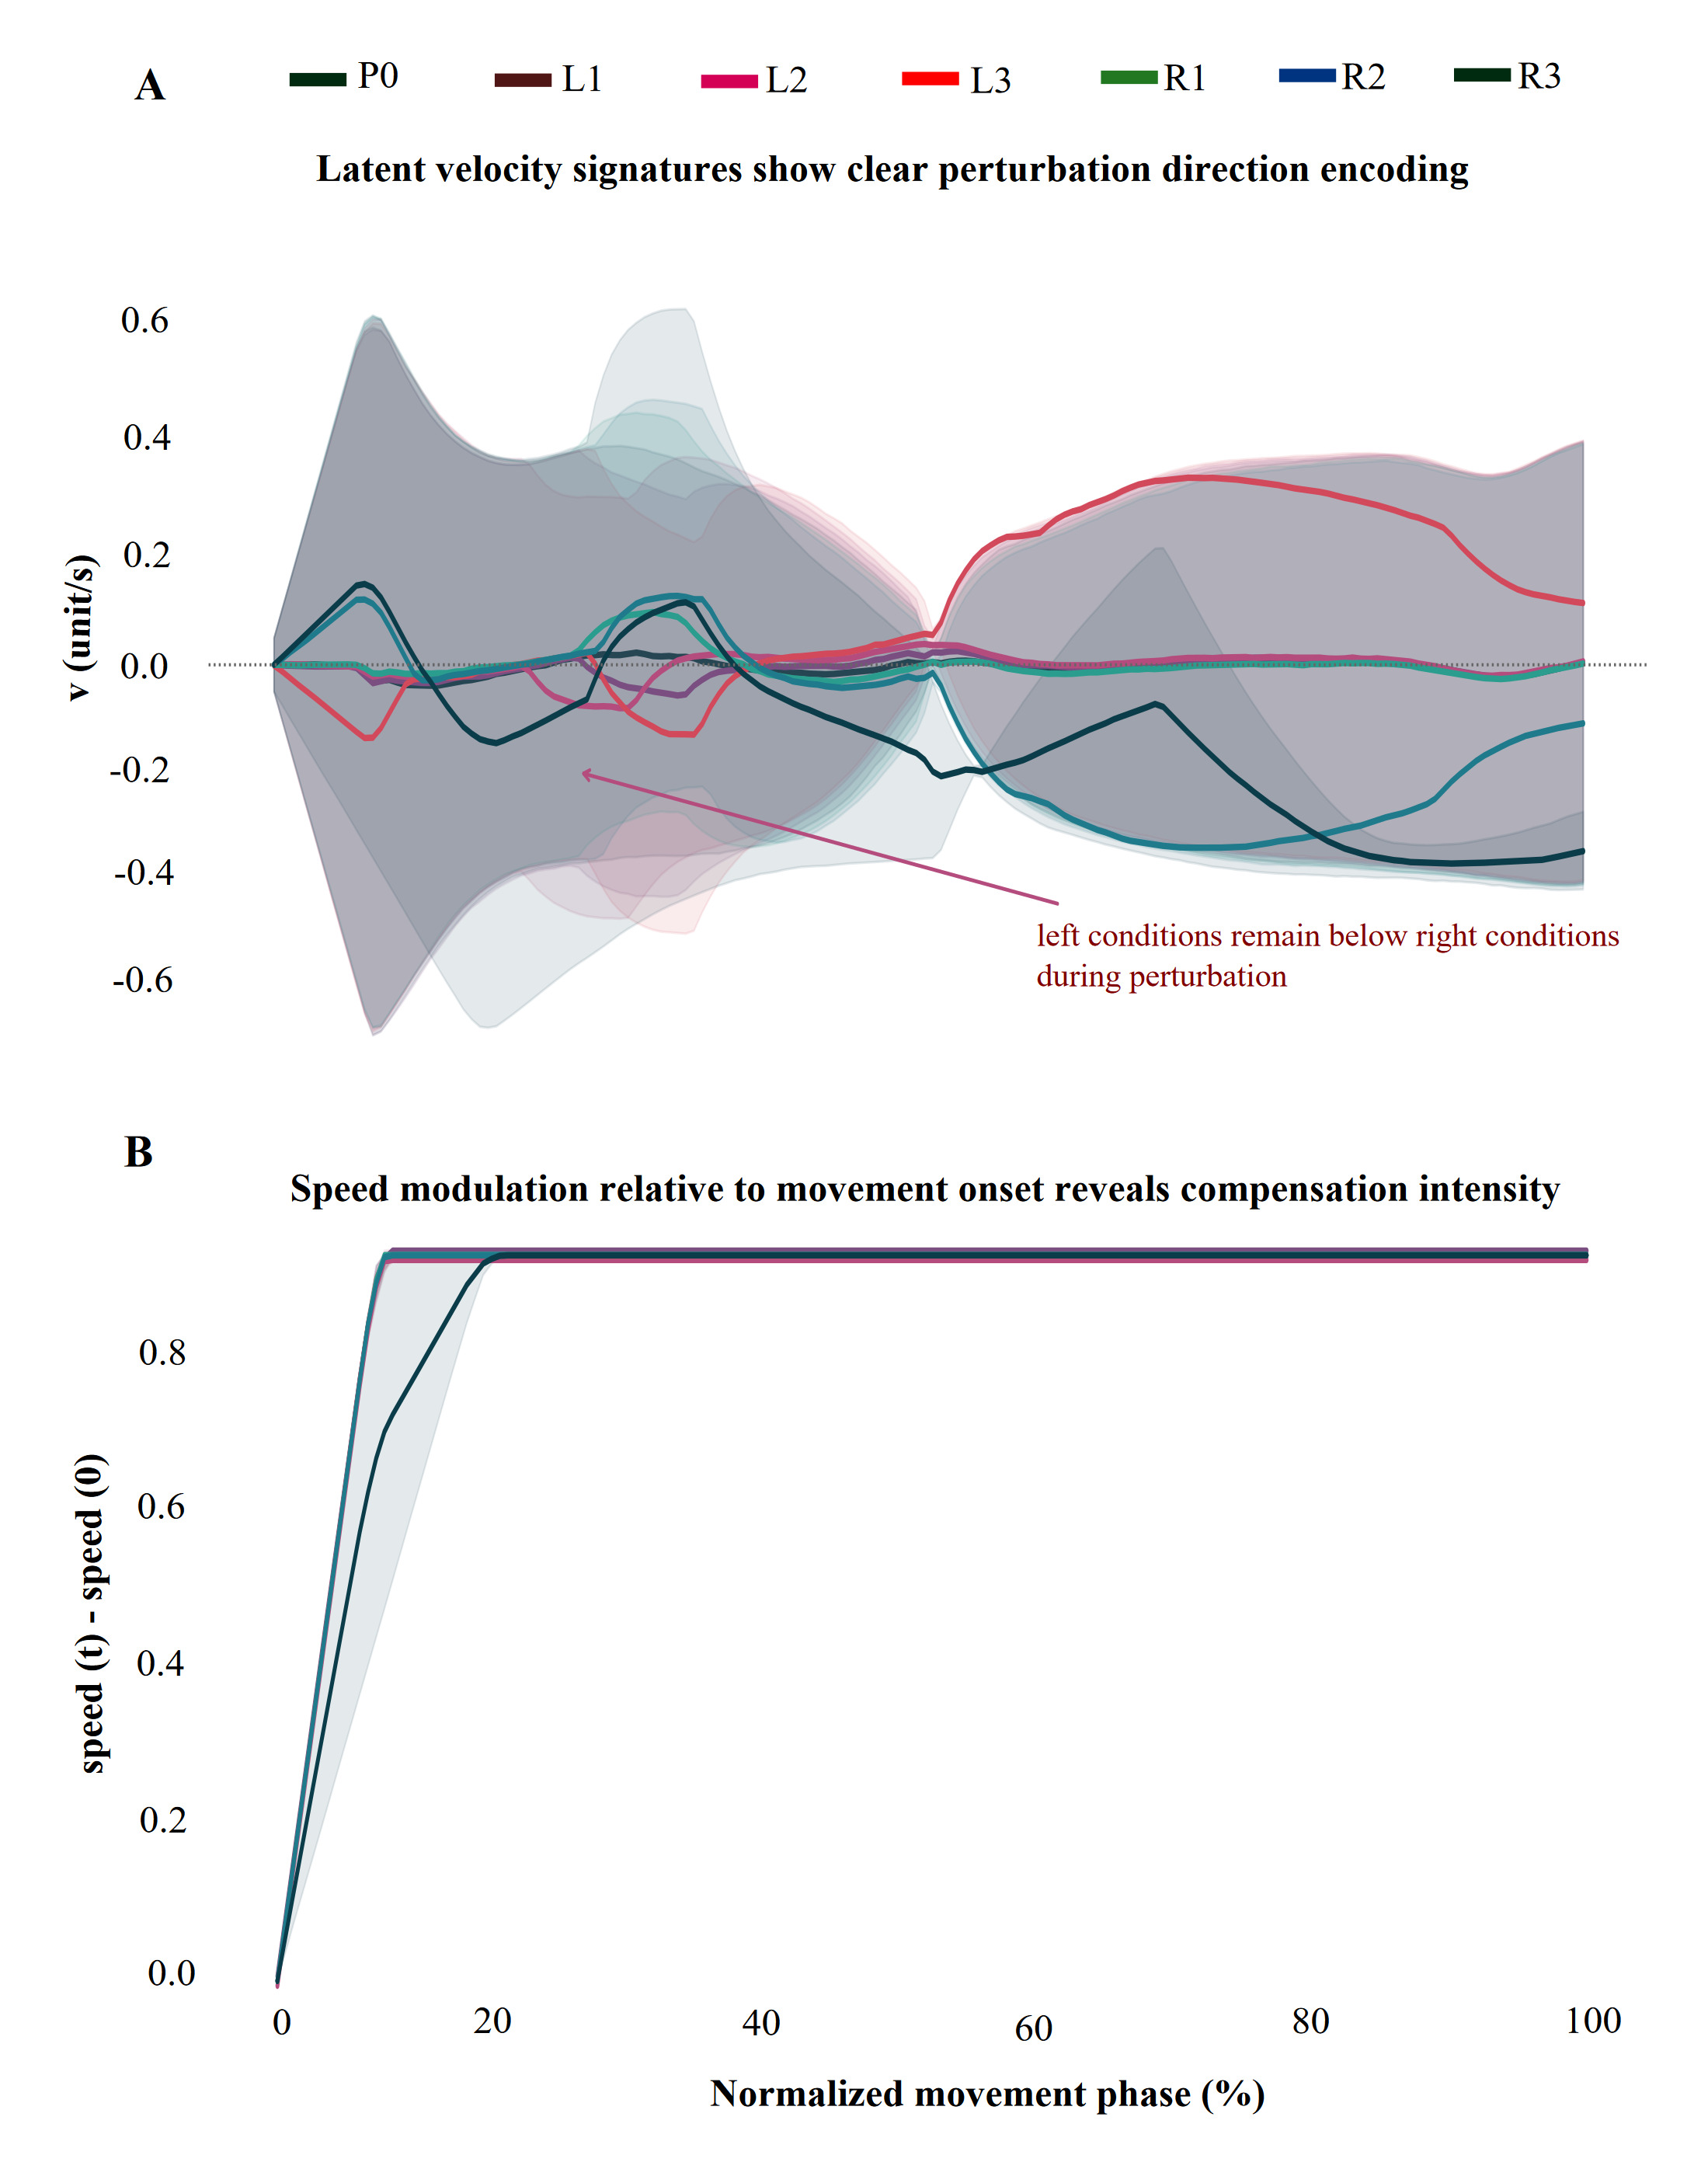
\includegraphics[width=0.80\linewidth]{fig3_velocity.png}
  \caption{\textbf{Velocity profiles reveal proportional perturbation
    encoding and preserved movement tempo.}
    \textbf{(A)}~Mean lateral velocity (horizontal component of velocity
    vector) over time, aligned to movement onset and averaged across all
    episodes within each condition. Shaded regions show $\pm$1\,SD,
    conveying trial-to-trial variability. Leftward conditions (L1--L3)
    drive the agent into negative lateral velocity (moving left), while
    rightward conditions (R1--R3) drive it into positive lateral velocity
    (moving right). Conditions diverge sharply during the perturbation
    window (timesteps 50--55, indicated by the vertical markers) and then
    partially reconverge, consistent with the generation of a proportional
    corrective response rather than a stereotyped binary reaction.
    Critically, the magnitude of lateral deflection scales with perturbation
    strength within each direction, suggesting a graded, analogue
    corrective mechanism.
    \textbf{(B)}~Total speed (Euclidean norm of the velocity vector)
    plotted as a function of normalised movement phase (0 = movement onset,
    100 = goal arrival). Speed rises steeply at movement onset, reaching
    a plateau that is maintained consistently across all seven perturbation
    conditions. This invariance of the speed profile confirms that the
    controller's response to lateral perturbations is expressed entirely
    through changes in movement direction rather than through changes in
    the overall pace of the movement, a dissociation that mirrors the
    kinematic signature of online feedback corrections in human arm
    movements \citep{Pruszynski2012,Nashed2014,FlashHogan1985}.}
  \label{fig:velocity}
\end{figure}

Panel~A shows that lateral velocity separated cleanly and systematically
by perturbation direction throughout the active perturbation window.
Leftward conditions produced negative lateral velocity; rightward
conditions produced positive lateral velocity; and in both directions the
magnitude of the lateral deflection scaled with perturbation strength.
Following the end of the perturbation window, conditions on the same side
partially reconverged toward the unperturbed trajectory, a signature that
the controller is generating a corrective force proportional to the
sensed displacement rather than a binary switch between pre-programmed
response modes.

Panel~B confirms that total movement speed was essentially invariant
across all seven conditions.
The controller increases speed rapidly at movement onset, reaches a plateau,
and maintains that plateau uniformly regardless of whether a perturbation is
applied or its magnitude and direction.
This dissociation between path geometry (which is modulated by
perturbation) and speed profile (which is not) is a hallmark of optimal
feedback control strategies in biological reaching
\citep{Todorov2002,Scott2004}.

Figure~\ref{fig:pca} shows the result of projecting the full 256-dimensional
hidden-layer activity onto its first two principal components across all
evaluation timesteps.

\begin{figure}[H]
  \centering
  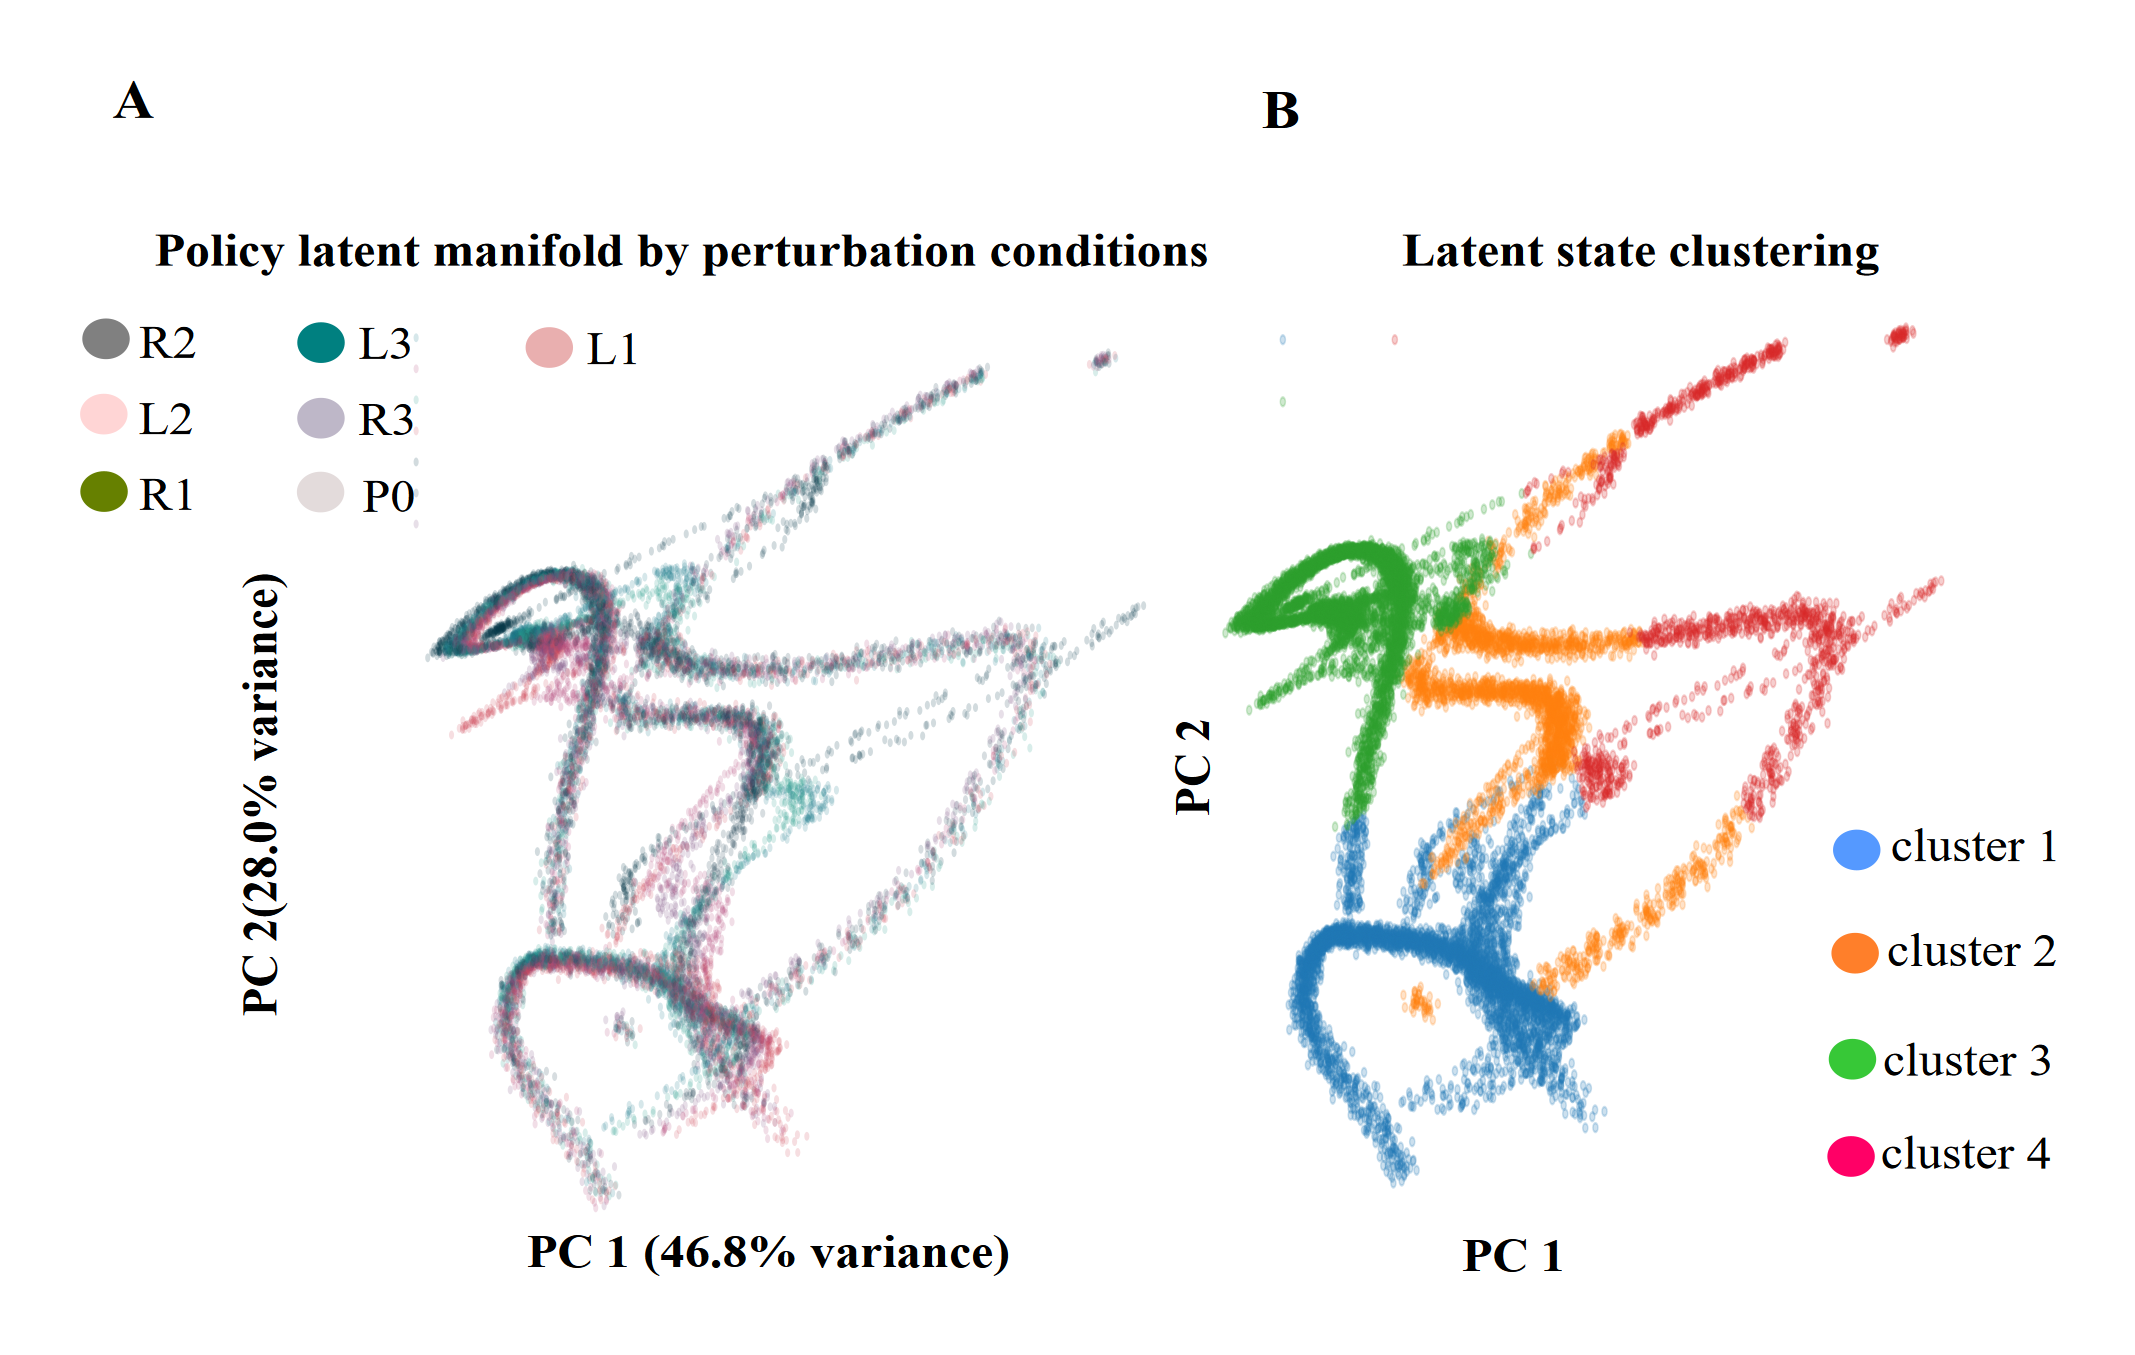
\includegraphics[width=0.88\linewidth]{fig4_pca.png}
  \caption{\textbf{Hidden-layer activity occupies a compact low-dimensional
    manifold with structure aligned to movement phases rather than to
    perturbation conditions.}
    Each point represents the 256-dimensional hidden-state vector at one
    evaluation timestep, projected onto the first two principal components
    of the entire evaluation dataset.
    \textbf{(A)}~Points are coloured by perturbation condition (see
    legend). The population activity traces a characteristic curved
    manifold whose gross shape is shared across all seven conditions.
    Conditions are not cleanly separated (they overlap substantially)
    but extreme conditions (particularly L3 and R3) occupy peripheral
    regions of the manifold that are partly distinct from the control
    and mild conditions.
    PC1 accounts for \PCAVarI{} of total variance, PC2 for \PCAVarII{};
    together they capture \PCAVarTotal{} of the variance in a
    256-dimensional network, demonstrating a high degree of dimensionality
    compression.
    \textbf{(B)}~The same projection coloured by $K$-means cluster label
    ($K=4$). Four spatially coherent clusters emerge that partition the
    manifold into anatomically distinct regions. These clusters are not
    condition-specific: each cluster contains timesteps from all seven
    perturbation conditions. Instead, the clusters likely correspond to
    phases of the reaching movement that are shared across conditions:
    for example, the initial approach to the perturbation zone
    (cluster~1), the active perturbation and correction epoch
    (cluster~2), the path around the obstacles (cluster~3), and the
    final approach to the goal (cluster~4). This phase-aligned structure
    closely resembles the sequential activation of distinct neural
    population states that has been documented in motor cortex during
    biological reaching movements \citep{Churchland2012,Shenoy2013}.}
  \label{fig:pca}
\end{figure}

Two findings emerge from this analysis.
The first is the degree of dimensionality compression.
Despite the policy network having 256 hidden units in its first layer,
\PCAVarTotal{} of the variance in the activation patterns collapses onto
just two dimensions.
This is a striking degree of compression, comparable in magnitude to
the low-dimensional manifold structure reported for motor cortex activity
during reaching in both non-human primates and humans
\citep{Churchland2012,Shenoy2013,Cunningham2014,Gallego2017,Sadtler2014,Elsayed2016}.
In both biological and artificial cases, the compression is not imposed
externally; it emerges from the structure of the learning problem itself.
When a system must produce a sequence of smooth, goal-directed movements,
the activity patterns across trials are necessarily correlated, and a
small number of principal directions can capture most of that shared
structure.

The second finding is the cluster organisation.
The $K$-means analysis with $K=4$ reveals four spatially coherent clusters
within the manifold.
These clusters do not separate perturbation conditions from one another;
rather, each cluster draws timesteps from all seven conditions.
This indicates that the clusters reflect something about the movement itself,
most likely its phase, rather than about the perturbation that is currently
acting.
This phase-aligned clustering parallels findings from motor cortex
recordings in biological reaching, where distinct neural population states
have been identified for the preparatory, movement initiation, and
movement completion epochs \citep{Churchland2012,Shenoy2013,Kaufman2014,Perich2018}.
We note that the choice of $K=4$ was not cross-validated; future work
with held-out datasets and multiple training seeds would be needed to
establish whether the four-cluster solution is a stable feature of the
representation.

Figure~\ref{fig:decoding} shows the confusion matrix from a linear
classifier trained on single-timestep hidden-layer activity to identify
the perturbation condition active on each trial.

\begin{figure}[H]
  \centering
  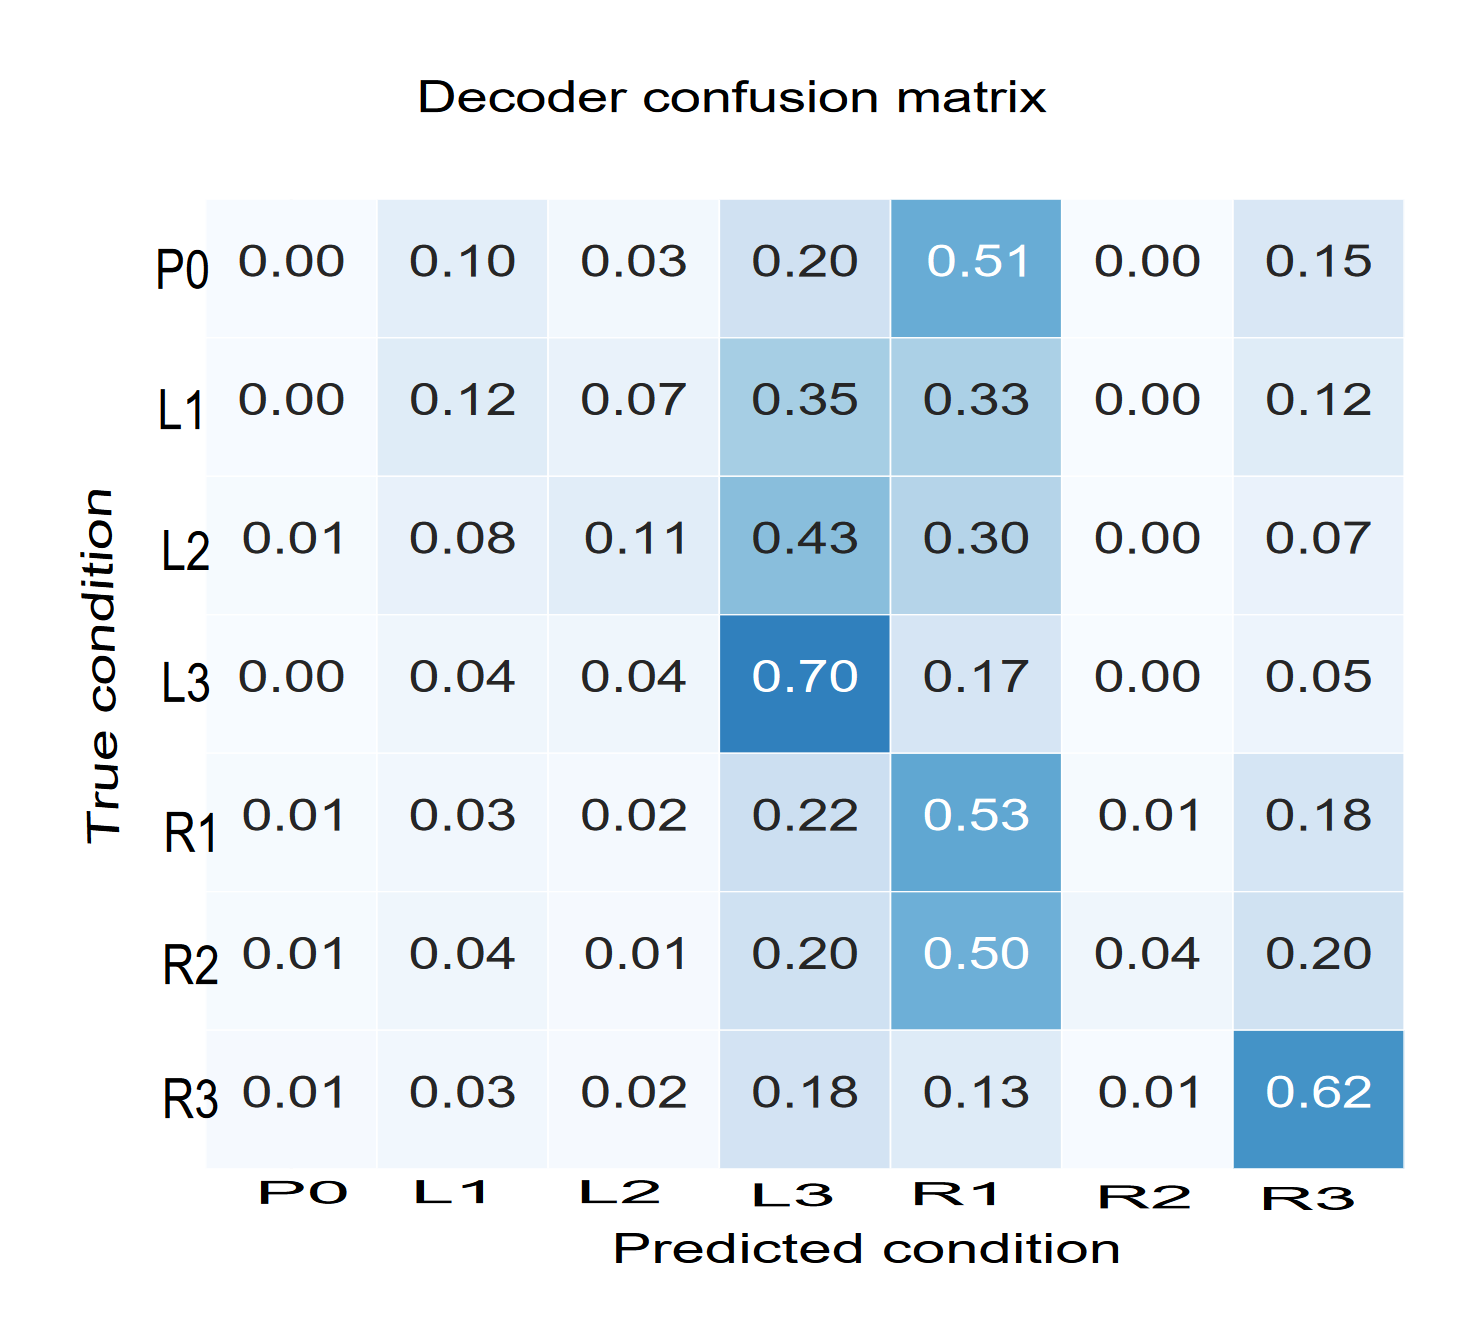
\includegraphics[width=0.56\linewidth]{fig5_decoding.png}
  \caption{\textbf{Linear decoding reveals that extreme perturbation
    conditions produce geometrically distinct population states, while
    mild conditions remain indistinguishable.}
    Rows of the confusion matrix correspond to the true perturbation
    condition for each timestep; columns correspond to the condition
    predicted by a multinomial logistic regression classifier trained on
    the 256-dimensional hidden-layer activation vector at that timestep.
    Diagonal entries indicate the proportion of
    timesteps from each true condition that were correctly classified.
    Importantly, the off-diagonal pattern reveals that misclassified
    timesteps are not randomly distributed: mild and control conditions
    (P0, L1, L2) are almost exclusively misclassified as L3 (the largest
    leftward perturbation), rather than being confused with rightward
    conditions. This systematic misclassification indicates that the
    latent states generated by mild perturbations are geometrically closer
    to the L3 region of the manifold than to any other condition,
    suggesting that similar corrective responses, regardless of the
    magnitude of the perturbation that elicited them, occupy similar
    regions of the latent space. The decoder's successful separation of
    extreme conditions (L3 and R3 achieved the highest diagonal values)
    confirms that the most behaviourally disruptive perturbations
    produce the most distinctive internal representations.}
  \label{fig:decoding}
\end{figure}

The classifier achieved its highest accuracy for the most extreme
perturbation conditions: the largest leftward impulse (L3) was correctly
identified on the majority of timesteps, and the largest rightward impulse
(R3) was correctly classified at a similarly high rate.
Moderate rightward conditions (R1, R2) were also decoded above chance.
The unperturbed control and mild leftward conditions (P0, L1, L2) were
decoded at near-chance levels, and when misclassified, they were
systematically assigned to L3 rather than to random conditions.
This is not a simple failure of the classifier; it is a feature of the
latent geometry.
Mild perturbations generate hidden states that occupy a region of the
manifold geometrically close to the L3 cluster, reflecting the fact that
mild corrections and large corrections that are ultimately successful
produce similar downstream activity.
What distinguishes them is the trajectory they took through the state
space to get there, not their momentary position.

The fact that a linear classifier can decode extreme conditions at all is
the more important result.
Perturbation context is encoded in the population activity in a structured,
geometrically accessible form: the relevant information is present in a
linear projection of the 256-dimensional activity vector.
This mirrors the finding from biological motor neuroscience that
target direction, perturbation magnitude, and trial outcome can all be
decoded with linear classifiers trained on motor cortex population activity
\citep{Churchland2012,Nashed2014,Oby2019,Georgopoulos1986,Sadtler2014}.

Figure~\ref{fig:learning} contextualises the representational findings
within the training dynamics of the controller.

\begin{figure}[H]
  \centering
  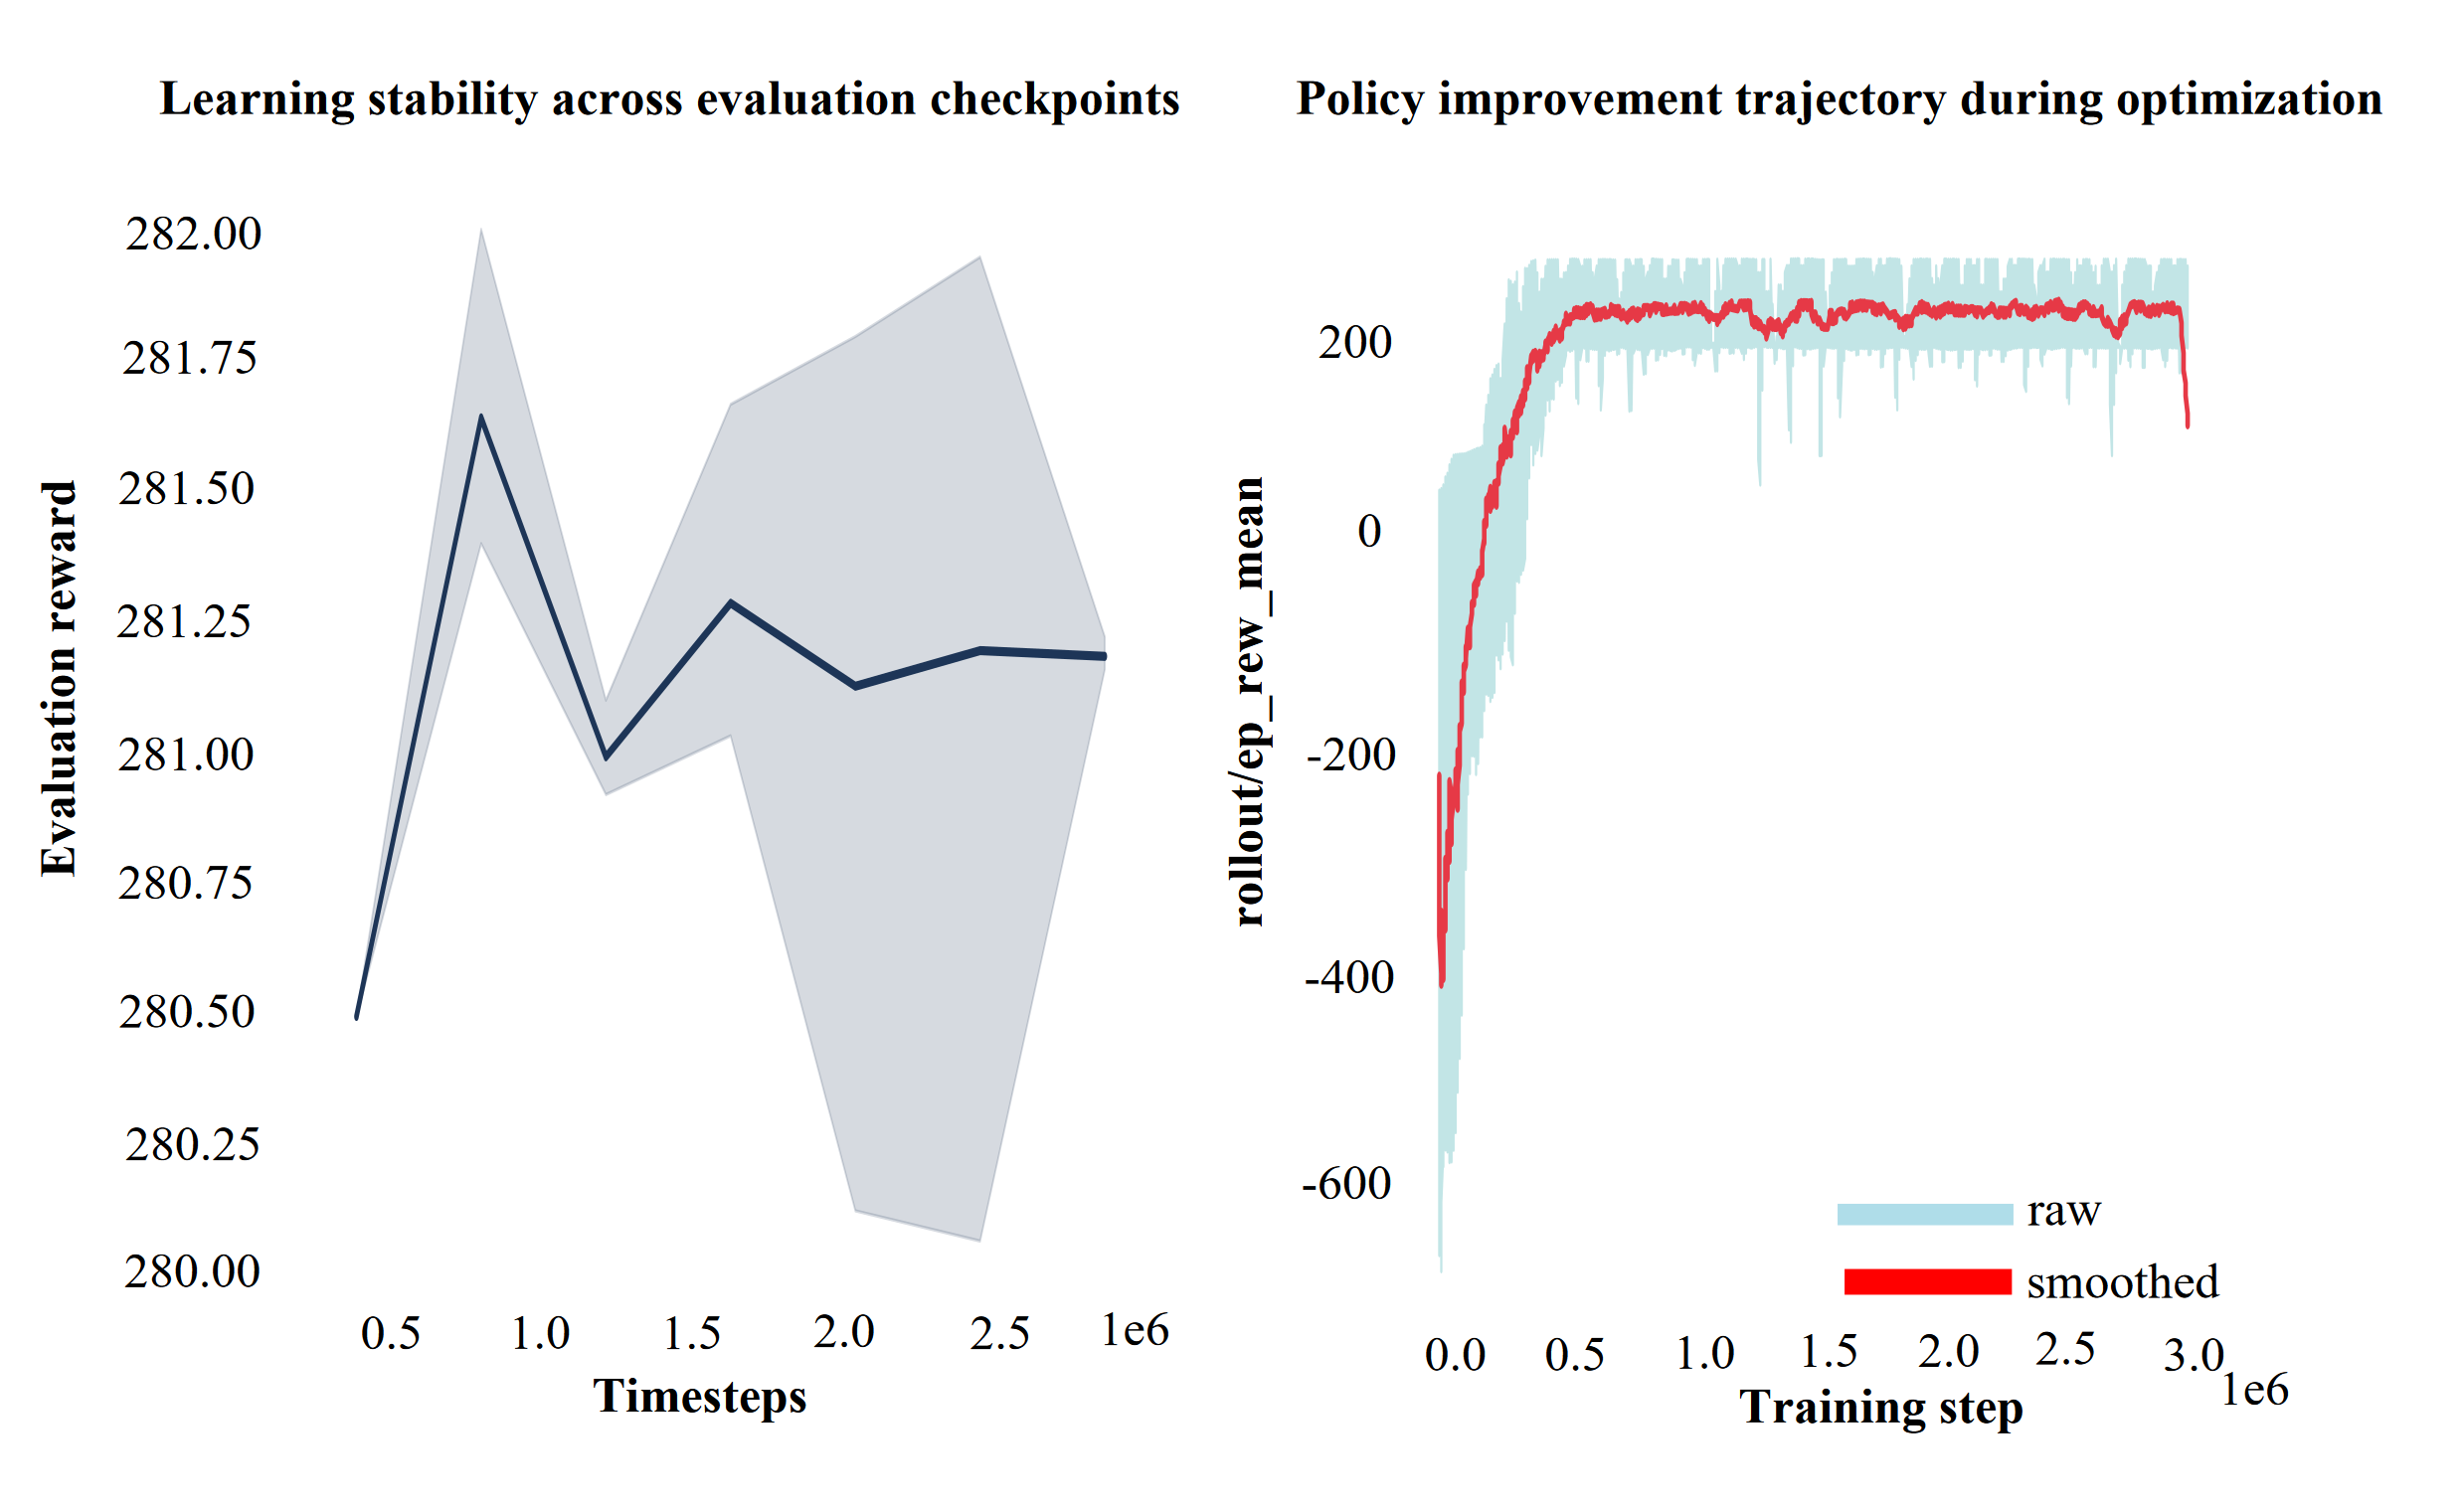
\includegraphics[width=0.82\linewidth]{fig6_learning.png}
  \caption{\textbf{The controller converges stably, validating the
    representational analyses as properties of a fully trained policy.}
    \textbf{(Left panel)}~Evaluation reward plotted across independently
    sampled checkpoints throughout training (mean $\pm$\,SD across all
    evaluation episodes at each checkpoint). The reward is tightly
    clustered around a high value once training has converged,
    demonstrating that performance is stable rather than oscillating, and
    that the policy extracted from any checkpoint after convergence will
    yield similar behaviour.
    \textbf{(Right panel)}~Raw per-episode rollout reward over the full
    $3\times10^6$-timestep training run (light blue), together with an
    exponential moving average (red) to reveal the learning trajectory.
    The policy improves rapidly from large negative initial rewards
    (reflecting early episodes in which the agent collides frequently)
    to a stable positive plateau within approximately the first
    $1\times10^6$ timesteps, after which performance remains stable
    without systematic degradation or catastrophic forgetting.
    The representations analysed in Figures~\ref{fig:pca}
    and~\ref{fig:decoding} were extracted from the converged policy
    (after $2\times10^6$ timesteps), ensuring that they reflect the
    learned representational structure rather than an artefact of
    incomplete training.}
  \label{fig:learning}
\end{figure}

\FloatBarrier

The training curve confirms that the controller learned the task efficiently
and converged to a stable solution within the first third of the training
budget.
After convergence, performance was tightly distributed across independently
sampled evaluation checkpoints, ruling out the possibility that the reported
behavioural and representational findings are artefacts of partial training
or of checkpoint selection.
The rapid initial improvement followed by a long stable plateau is
characteristic of well-tuned PPO training on continuous-control problems
and is consistent with the training dynamics reported for similar
obstacle-avoidance and reaching tasks in the RL literature
\citep{Raffin2021StableBaselines3,Schulman2017}.

%==============================================================
\section{Discussion}
%==============================================================

This study asked whether a controller trained by reinforcement learning
to perform adaptive obstacle avoidance develops internal representations
that are interpretable using the analytical framework of systems motor
neuroscience.
We find consistent evidence that it does: the hidden-layer activity of
a converged PPO policy organises into a compact low-dimensional manifold
with phase-aligned cluster structure, encodes kinematic variables in a
distributed, graded way, and contains linearly readable information about
perturbation context that is most distinct for the most behaviourally
demanding conditions.
We discuss these findings in relation to biological motor control,
consider what they reveal about the controller's failure modes, and
acknowledge the limitations that bound their generality.

\paragraph{Behavioural adaptation mirrors biological feedback correction.}

The pattern of behavioural adaptation, characterised by robust performance
under mild perturbations, progressive degradation under stronger ones, and
adaptation expressed through path correction rather than speed modulation,
is qualitatively consistent with the kinematic signatures of online feedback
corrections in human reaching.
In biological reaching, the primary motor cortex and premotor areas
generate rapid, graded corrective responses to unexpected force perturbations
that reshape the movement path without systematically altering movement
speed \citep{Pruszynski2012,Nashed2014,FlashHogan1985,Scott2004,Dimitriou2013,Shadmehr1994,Diedrichsen2010}.
The PPO controller exhibits precisely this dissociation: it modulates
path geometry in proportion to the applied force while keeping the overall
movement tempo constant across all seven conditions (Figure~\ref{fig:velocity}B).

We are careful not to overstate this correspondence.
The point-mass dynamics are far simpler than those of a biological limb;
the controller has no muscle mechanics, no proprioceptive noise, and no
time delays in sensory feedback.
The PPO policy was optimised for cumulative reward, not for kinematic
smoothness or biological realism.
Nevertheless, the convergence of the kinematic signature of proportional
lateral deflection with preserved speed is consistent with the computational
principles of optimal feedback control (OFC), which predicts that
well-adapted controllers should correct task-relevant errors while
leaving task-irrelevant variables unchanged \citep{Todorov2002,Todorov2009,Franklin2011,WolpertGhahramani2000}.
Under OFC, speed is a task-irrelevant variable when a lateral perturbation
is applied; correcting it would waste motor resources without improving
goal attainment.
The PPO controller, trained purely by reward, appears to discover the same
principle implicitly.

The direction-dependent asymmetry in robustness (rightward conditions
failing at lower magnitudes than leftward) is a geometric consequence of
the learned trajectory.
It is a useful reminder that performance under perturbation is not solely
a property of the controller; it is a joint property of the controller and
the specific task geometry in which it operates.
Future work with symmetric corridors and bidirectional reward shaping
could establish whether the asymmetry can be removed without sacrificing
overall performance.

\paragraph{Low-dimensional latent structure and its biological parallel.}

The finding that \PCAVarTotal{} of the variance in a 256-unit network
collapses onto two dimensions is the most theoretically significant result
of this study, because it was not imposed by the network architecture.
The MLP has no bottleneck layer, no regularisation that explicitly
penalises high-dimensional representations, and no biological constraints.
Yet the activity self-organises into a highly compressed subspace.

The same phenomenon has been documented repeatedly in motor cortex.
Recordings from hundreds of neurons during reaching show that most of the
variance in the neural activity lives in a subspace of far lower dimension
than the number of recorded cells
\citep{Churchland2012,Shenoy2013,Cunningham2014,Gallego2017}.
The interpretation offered in the biological literature is that the
repetitive, structured nature of movement, which proceeds through a
stereotyped sequence of phases regardless of specific kinematics, forces
the neural population into a low-dimensional orbit through activity space.
Our results suggest that the same logic applies to artificial controllers:
because all reaching movements share a common temporal structure
(acceleration, obstacle passage, deceleration toward goal), the hidden
states across all trials are necessarily correlated, and a small number
of principal components suffice to capture that shared structure.

The four-cluster decomposition of the manifold (Figure~\ref{fig:pca}B)
provides a complementary view.
The clusters partition the manifold spatially, and because they do not
separate perturbation conditions they most naturally correspond to movement
phases: the approach to the perturbation zone, the active perturbation
and correction epoch, the passage around the obstacles, and the final
approach to goal.
This phase-aligned clustering is consistent with the sequential activation
of distinct neural population states documented in motor cortex during
biological reaching \citep{Churchland2012,Shenoy2013,Kaufman2014,Elsayed2016,Georgopoulos1986}.
We again note that the choice of $K=4$ was not cross-validated; the number
of clusters and their boundaries could shift across training seeds or
evaluation datasets.

\paragraph{What the decoder tells us about internal organisation.}

The systematic pattern of decoder performance, which was accurate for
extreme conditions and near-chance for mild ones, with mild conditions
systematically misclassified as L3 rather than as random conditions,
carries a specific message about the geometry of the latent space.
It means that the hidden states generated by mild perturbations, while
physically distinct in the external world, produce internal
representations that are more similar to those generated by large
perturbations than to those generated by the control condition.
This is ecologically sensible: a small perturbation that the controller
handles with a small correction generates a hidden state trajectory that
passes close to the L3 region of the manifold, because a large
perturbation that the controller handles well with a large correction
passes through the same region.
The relevant variable that separates these cases is not the instantaneous
manifold position but the magnitude of the preceding displacement and
corrective force; this information is carried in the trajectory through
state space rather than in any single point.

This interpretation has a direct parallel in biological motor
neuroscience.
Studies of motor cortex activity during online reaching corrections show
that the decodability of perturbation magnitude improves substantially
when the decoder is given a temporal window of population activity rather
than a single snapshot \citep{Nashed2014,Churchland2012,Sadtler2014,Perich2018}.
The same principle likely applies here: the latent state at any single
timestep is not a sufficient summary of the perturbation history, but the
sequence of latent states over the correction epoch likely is.
Future work with recurrent or temporal decoding approaches could test this
directly.

\paragraph{Limitations.}

Several constraints bound the generality of these conclusions.

\textit{Single training seed.}
All results are from a single PPO training run.
We cannot quantify how much of the reported structure (degree of
dimensionality compression, number of clusters, pattern of decoder
performance) varies across seeds.
Systematic multi-seed experiments are needed to establish which features
are stable properties of the learning algorithm and task, and which are
idiosyncratic to this particular run.

\textit{Simplified environment.}
The two-dimensional point-mass environment abstracts away several features
that are present in biological reaching: three-dimensional kinematics, muscle
mechanics, sensory noise, neural delays, and the memory of past perturbations
(since the MLP has no recurrence).
Whether the representational organisation we describe here would persist
in richer, more biologically realistic environments is an open question.

\textit{Feedforward architecture.}
The absence of recurrence means that the controller processes each
timestep's observation independently.
It cannot explicitly maintain an estimate of the perturbation that was
applied in previous timesteps, which may limit its capacity to generate
temporally coherent corrections under conditions where the perturbation
is unpredictable.

\textit{Descriptive analyses.}
PCA and linear decoding identify and characterise structure; they do not
establish which specific hidden units or circuits cause the behaviour.
Causal interventions would be needed to move from description to mechanism.

\textit{Use of AI tools.}
Large language models were used to support text editing, proofreading,
debugging, and \LaTeX\ formatting.

\paragraph{Connecting to biological motor systems.}

Taken together, our results contribute to a growing body of evidence that
the organisational principles of biological motor populations, namely compact
manifold geometry, phase-structured latent dynamics, distributed and graded
encoding of kinematic variables, and linear decodability of task-relevant
context, are not unique features of biological neural circuits.
They can emerge spontaneously in artificial controllers trained by
reinforcement learning, without any architectural constraints or
biological supervision
\citep{Churchland2012,Gallego2017,Oby2019,Crevecoeur2019,Silver2016,Haarnoja2018,Mnih2015DQN}.
This convergence has implications in both directions.

For motor neuroscientists, it suggests that the low-dimensional, phase-structured
representations observed in motor cortex may be a computationally preferred
solution to the general problem of generating smooth, goal-directed
movements under uncertainty, a solution that emerges from optimisation
pressure rather than from the specific biophysical properties of cortical
circuits \citep{Franklin2011,WolpertGhahramani2000,Rizzolatti2001,Berniker2011}.
This raises the possibility of using well-characterised RL controllers
as computational models for generating testable predictions about
population dynamics in motor cortex, particularly under novel perturbation
conditions that are difficult to study in biological experiments.

For engineers and clinicians working on assistive and rehabilitation
technologies, the framework demonstrates that population-style analysis
of artificial controller hidden states can reveal mechanistic information
that task-success metrics alone cannot.
Understanding which internal states predict failures, and specifically
which latent configurations mark the transition from successful correction
to collision, could provide actionable targets for
improving controller robustness or for designing failure-detection modules
that flag high-risk states before they produce behavioural errors.

%==============================================================
\section{Conclusion}
%==============================================================

We trained a PPO controller to navigate a reaching-inspired
obstacle-avoidance task and probed it with graded lateral force
perturbations spanning both directions, then analysed the internal
representations of the converged policy using the population-level
toolkit of motor neuroscience.

The controller adapted to moderate perturbations through lateral path
corrections that preserved movement speed, and its robustness degraded
asymmetrically under strong rightward disturbances as a consequence of
the geometry of the learned corridor trajectory.
The hidden-layer activity organised into a compact low-dimensional manifold,
capturing the large majority of population variance in just two principal
components, with four phase-aligned clusters shared across all perturbation
conditions.
A linear decoder trained on single-timestep hidden-layer activity could
separate extreme perturbation conditions, while mild conditions were
geometrically indistinguishable from one another and from the control,
reflecting similar corrective strategies rather than similar external
forces.

These findings demonstrate that reward-driven learning generates internal
representations with organisational properties, namely low dimensionality,
phase structure, graded kinematic encoding, and linear decodability of task
context, that are consistent with those documented in biological motor cortex.
Population-style analysis of RL controllers provides an analytical window
that extends beyond behavioural evaluation, offering a path toward
understanding not just whether an adaptive controller succeeds, but
mechanistically why it sometimes fails.

Future work will extend this framework to recurrent architectures that
can maintain temporal estimates of perturbation history, to richer
three-dimensional environments with contact dynamics, and to systematic
multi-seed experiments that characterise the variability of the
representational structure across training runs.
We also intend to apply these methods to rehabilitation-inspired control
problems, where linking internal neural representations to behavioural
recovery outcomes could contribute to the development of more
interpretable, trustworthy assistive technologies.

%==============================================================
\section*{Acknowledgments}
%==============================================================

This work was supported in part by the Connected Minds Program,
Canada First Research Excellence Fund,
Grant No.~CFREF-2022-00010.

\bibliographystyle{unsrtnat}
\bibliography{references}

\end{document}
